\documentclass[10pt, a4paper]{scrartcl}

\usepackage{vorschule}
\usepackage[
	typ=ab,
	fach=Informatik,
	lerngruppe={Q1-LK} ,
	nummer=8,
	module={Symbole,Lizenzen},
	seitenzahlen=keine,
	farbig,
	lizenz=cc-by-nc-sa-4,
]{schule}

\usepackage[
	kuerzel=Ngb,
	reihe={Automaten und formale Sprachen} ,
	version={2021-03-07} ,
]{ngbschule}

\author{J. Neugebauer}
\title{Kellerautomaten}
\date{\Heute}

\setzeAufgabentemplate{ngbnormal}

\usepackage{FLaAL}
\usepackage{qrcode}
\usepackage{subcaption}

\DeclareCaptionSubType*[alph]{figure}
\captionsetup[subfigure]{labelformat=simple,labelsep=colon}

\renewcommand{\qrhinweis}[1]{%
	\begin{wrapfigure}[4]{r}{0pt}
		\qrcode[height=1cm]{#1}
	\end{wrapfigure}%
}

\begin{document}
\ReiheTitel

Reguläre Sprachen haben ihre Grenzen. Die Sprache $a^nb^n, n\geq 0$ kann nicht durch einen endlichen Automaten akzeptiert werden und wir können auch keine reguläre Grammatik konstruieren. Die Sprache ist also nicht regulär, sondern \emph{kontextfrei}. Um einen Automaten zu konstruieren, der eine kontextfreie Sprache akzeptiert, müssen wir das Automatenmodell erweitern. 

Das Grundproblem: \emph{Ein endlicher Automat kann nicht zählen!} Er kann sich nicht merken, wie viele $a$ schon gekommen sind, um entsprechend viele $b$ abzuzählen. Wir brauchen also eine Struktur, die uns das Zählen erlaubt und diese finden wir im \emph{Keller}.

\begin{infobox}
Ein \emph{nichtdeterministischer Kellerautomat} (NKA) wird als 7-Tupel $A = (Q, \Sigma, K, \delta, q_0, \#, F)$ definiert:
\begin{itemize}
	\item $Q$ ist die (endliche) Menge von Zuständen des Automaten.
	\item $\Sigma$ ist das Eingabealphabet.
	\item $K$ ist das Kelleralphabet.
	\item $\delta: Q\times (\Sigma\cup \{\varepsilon\}) \times K\rightarrow \mathcal P(Q \times K^{*})$ ist die Übergangsfunktion.
	\item $q_0\in Q$ ist der Startzustand.
	\item $\#\in K$ ist das Startsymbol des Kellers.
	\item $F\subset Q$ ist die Menge der Endzustände.
\end{itemize}
\end{infobox}

\begin{wrapfig}
\begin{wrapfigure}[12]{r}{0pt}
	\centering
	%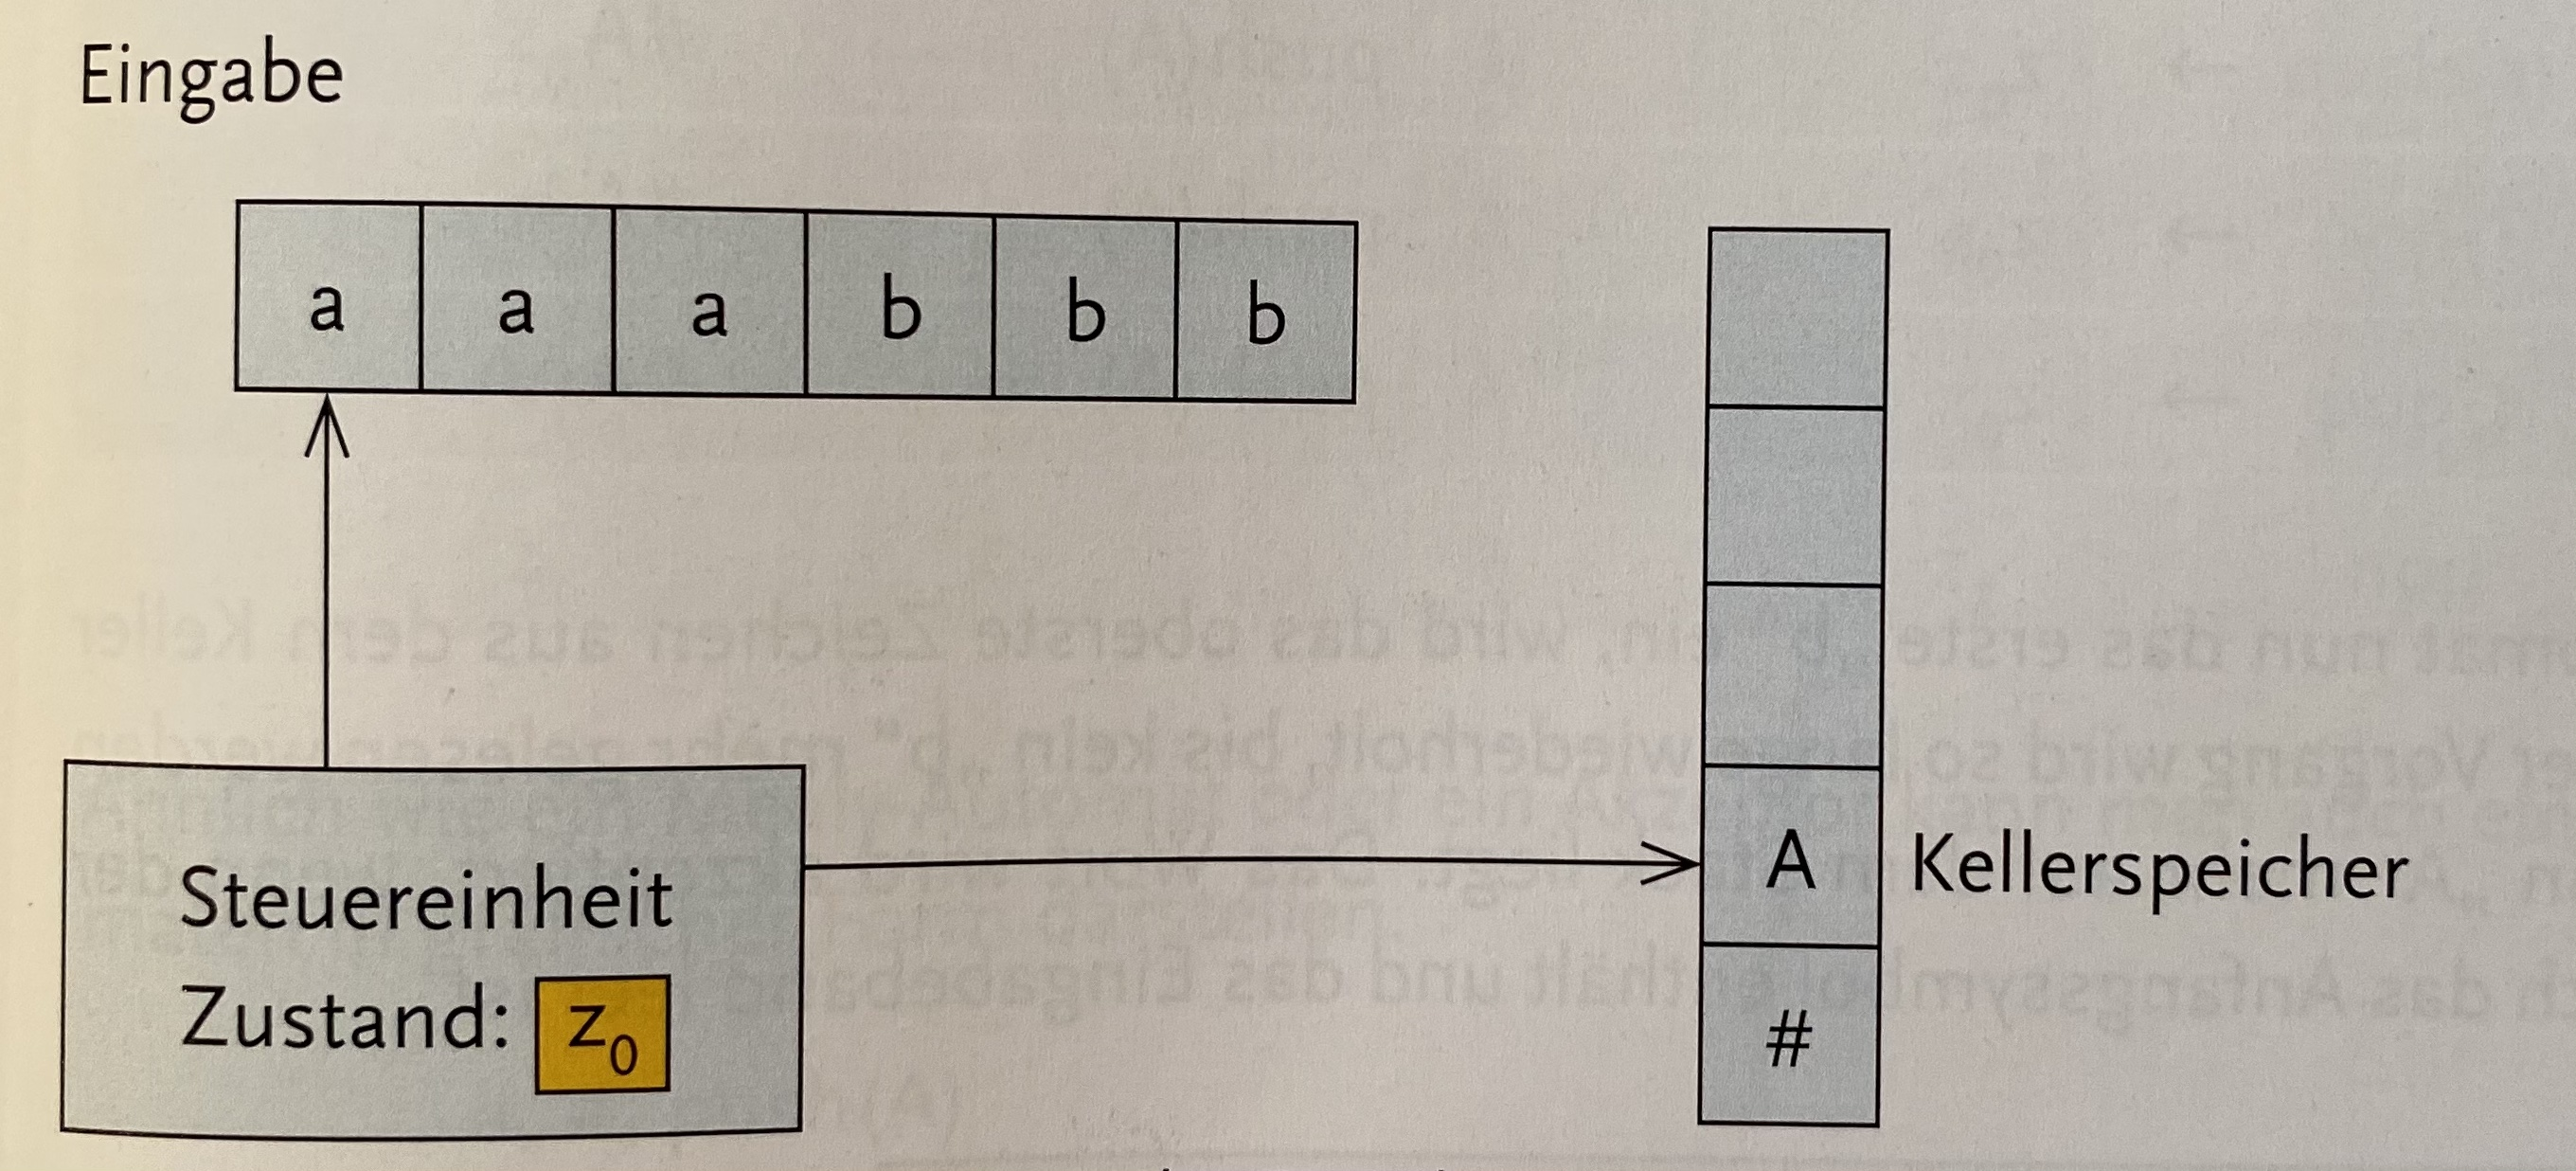
\includegraphics[width=6cm]{Q1-LK-AB.08-Kellerautomaten.jpeg}
	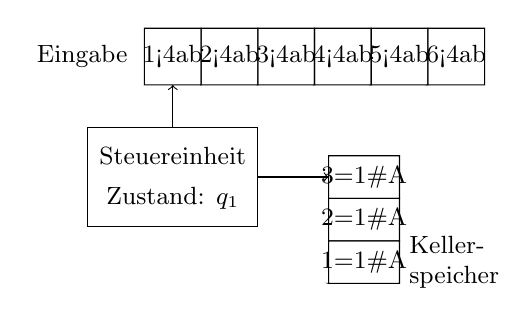
\begin{tikzpicture}[scale=.9]
		\draw (0,0) |- +(2.4,1.4) |- cycle;
		\foreach \i in {1,...,6} {
			\draw (\i*.8,2) |- +(.8,.8) |- cycle;
			\node[font=\small] at ({.4+\i*.8},2.4) {\ifthenelse{\i<4}{a}{b}};%
		}
		\foreach \i in {1,...,3} {%
			\draw (3.4,{-1.4+\i*.6}) |- +(1,.6) |- cycle;
			\node[font=\small] at (3.9,{-1.1+\i*.6}) {\ifthenelse{\i=1}{\#}{A}};%
		}
		\draw[->] (2.4,.7) -- (3.4,.7);
		\draw[->] (1.2,1.4) -- (1.2,2);
		
		\node[font=\small] at (1.2,1) {Steuereinheit};
		\node[font=\small] at (1.2,.4) {Zustand: $q_1$};
		\node[font=\small,anchor=west,text width=1cm] at (4.4,-0.5) {Keller\-speicher};
		\node[font=\small,anchor=east] at (.7,2.4) {Eingabe};
	\end{tikzpicture}
	\caption{Schematische Darstellung eines Kellerautomaten}
	\label{abb:schema_nka}
\end{wrapfigure}
Schematisch kann man sich einen Kellerautomaten wie in \prettyref{abb:schema_nka} vorstellen.

Jeder Übergang liest nun nicht mehr nur einen Buchstaben aus dem Eingabealphabet, sondern auch einen Buchstaben aus dem Kelleralphabet: Den obersten Buchstaben auf dem Keller. Das Kellerstartsymbol $\#$ liegt zu Beginn im Keller. Wenn es gelesen wird, dann gilt der Keller als leer.

Zur Darstellung des Übergangsgraphen erweitern wir die Darstellung eine endlichen Automaten um das Kelleralphabet:
\end{wrapfig}

\begin{figure}[h]
	\centering
    \begin{transitiongraph}[pa]
	        \state[s]{q0}{0}{0}
	        \state{q1}{30}{0}
	        \state[f]{q2}{60}{0}
	        \transition{q0}{q0}{\#,a,A\#;A,a,AA}
	        \transition{q0}{q1}{A,b,}
	        \transition{q1}{q1}{A,b,}
	        \transition{q1}{q2}{\#,,}
	    \end{transitiongraph}
	\caption{Kellerautomat zur Sprache $L_K= a^nb^n$ (Klammersprache).}
	\label{abb:nka_klammern}
\end{figure}

Ein Übergang hat nun die Form $(X, Y): Z^{*}$, wobei $X\in K$, $Y\in \Sigma$ und $Z\in K$ sind. Zu beachten ist, dass die Folge von Kellersymbolen $Z^{*}$ \emph{von rechts nach links} auf den Keller gelegt werden. Für $Z = \varepsilon$ wird nichts auf den Keller gelegt. Da immer das oberste Kellersymbol gelesen wird, wird also ein Buchstabe vom Keller entfernt!

\newpage

\begin{aufgabe}
\label{aufg:nka-klammern}
Baue den Kellerautomaten zur Klammersprache in \prettyref{abb:nka_klammern} in FLACI nach und teste ihn.
\end{aufgabe}

\begin{aufgabe}
\label{aufg:nka-klammern2}
In der Regel ist nicht nur die Verschachtelung von Klammerpaaren ineinander erlaubt, sondern auch mehrere verschachtelte Klammerpaare hintereinander.

\begin{teilaufgaben}
	\teilaufgabe
	Erweitere den Klammerautomaten aus \prettyref{aufg:nka-klammern} zur Sprache
	\[ L_{K2} = (L_K)^{*} = (a^{n_i}b^{n_i})^{m}, n_i\geq 1, m\geq 0, i = 1,...,m \]
	Gültige Worte sind zum Beispiel: $aaabbbaabb$, $ababab$, $aabbaabb$.

	\teilaufgabe
	Erweitere den NKA $L_{K2}$ zur Sprache $L_{K3}$, die beliebige gültige Klammerausdrücke erkennt. Im Gegensatz zu $L_{K2}$ sind dann auch Worte wie $aababb$ oder $aaabaababbabbb$ gültig. (Es dürfen also neue Klammerpaare beginnen, bevor alle Klammern geschlossen wurden.)
\end{teilaufgaben}
\end{aufgabe}

\begin{aufgabe}
\label{aufg:nka-uebungen}
Entwickle in FLACI einen NKA für die Sprachen $L_4$ bis $L_6$:

\begin{itemize}
	\item[$L_4$]$ = a^n(a|b|c)^n, n \geq 1$
	\item[$L_5$]$ = \{ w_1 a w_2 | w_1\text{ und }w_2\text{ sind gleichlange Worte über }\{1,0\} \}$
	\item[$L_6$]$ = a^nb^m, 0 \leq a < b$
\end{itemize}

Gib auch jeweils die formale Definition der Automaten als 7-Tupel an.
\end{aufgabe}

\begin{aufgabe}
\label{aufg:grammatik-uebungen}

Erstelle zu den Sprachen $L_4$, $L_5$ und $L_6$ aus \prettyref{aufg:nka-uebungen} jeweils eine kontextfreie Grammatik, die die Sprache erzeugt.
\end{aufgabe}

\begin{aufgabe}
\label{aufg:grammatik-rechenterme}
$G_{RE} = (N,T,S,P)$ ist die rechtsreguläre Grammatik für Rechenterme vom Arbeitsblatt 5, mit den in \prettyref{abb:grammatik-rechenterme} gezeigten Produktionen (zur Vereinfachung wird die Kurzschreibweise $0..3 B$ für $0B|1B|2B|3B$ genutzt).

Erweitere $G_{RE}$ zu einer kontextfreien Grammatik, die auch Terme mit korrekten Klammerausdrücken erlaubt.
\end{aufgabe}

\begin{figure}[h]
	\begin{subfigure}{.5\textwidth}
		\begin{align*}
		S &\rightarrow 0 A \,|\, 1..9 B \,|\, \varepsilon \\
		A &\rightarrow . C\,|\, +E \,|\, - E \,|\, \cdot E \,|\, : E \,|\, \varepsilon \\
		B &\rightarrow . C \,|\, 0..9 B \,|\, +E \,|\, - E \,|\, \cdot E \,|\, : E \,|\, \varepsilon \\
		C &\rightarrow 0..9 D \\
		D &\rightarrow 0..9 D \,|\, +E \,|\, - E \,|\, \cdot E \,|\, : E \,|\, \varepsilon \\
		E &\rightarrow 0 A \,|\, 1..9 B
		\end{align*}
		\caption{Produktionen von $G_{RE}$.}
		\label{abb:grammatik-rechenterme}
	\end{subfigure}%
	\begin{subfigure}{.5\textwidth}
		\begin{transitiongraph}[pa]
			\state[s]{q0}{0}{0}
			\state{q1}{25}{0}
			\state[f]{q2}{50}{0}
			\transition{q0}{q0}{\#,a,A\#;\#,b,B\#;A,a,AA;A,b,BA;B,a,AB;B,b,BB}
			\transition{q0}{q1}{A,a,;B,b,}
			\transition{q1}{q2}{\#,,\#}
			\transition{q1}{q1}{A,a,;B,b,}
		\end{transitiongraph}
		\caption{Übergangsgraph eines NKA.}
		\label{abb:nka-palindrom}
	\end{subfigure}
\end{figure}

\begin{aufgabe}
\label{aufg:nka-palindrom}
Welche Sprache beschreibt der Kellerautomat zum in \prettyref{abb:nka-palindrom} gezeigten Übergangsgraphen?
\end{aufgabe}

\end{document}